\documentclass[conference]{IEEEtran}

\usepackage{cite}
\usepackage{amsmath,amssymb}
\usepackage{graphicx}
\usepackage{hyperref}

\begin{document}

\title{AI-Assisted Programming in Software Engineering: A Systematic Literature Review on Capabilities, Productivity, and Code Quality}

\author{
\IEEEauthorblockN{L.F. Guevara-Chávez}
\IEEEauthorblockA{
School of Engineering and Science \\
Tecnológico de Monterrey \\
Tampico, México \\
leon.guevara@tec.mx}
}

\maketitle

\begin{abstract}
The rapid adoption of AI-assisted programming tools, particularly those based on large language models (LLMs), has significantly transformed software development practices. While these tools promise substantial productivity gains, existing evidence remains fragmented and, in some cases, contradictory. This study presents a systematic literature review of empirical research published between 2020 and 2026, synthesizing findings from controlled experiments, large-scale observational studies, industrial deployments, and qualitative investigations.

The analysis integrates evidence across multiple dimensions, including productivity, code quality, technical debt, human--AI interaction, cognitive load, organizational impact, economic viability, and developer perception. Results indicate that AI-assisted programming consistently increases development output; however, these gains are often accompanied by trade-offs, such as higher verification effort, increased technical debt, and shifts in maintenance responsibilities. Furthermore, the effectiveness of these tools is highly contingent on factors such as developer experience, intensity of adoption, and the quality of human--AI interaction, particularly in iterative prompting and validation processes.

The findings also reveal a notable gap between perceived and actual productivity, as well as the importance of cognitive and sociotechnical factors, including trust calibration and community-driven heuristics, in shaping tool usage. From an economic perspective, AI-assisted development can be viable under appropriate conditions, although it introduces additional costs related to training, supervision, and integration.

Overall, this study advances the understanding of AI-assisted programming as a multifaceted, socio-technical phenomenon. Rather than acting as a simple productivity enhancer, these tools reshape how developers work, collaborate, and make decisions, highlighting the need for balanced adoption strategies and further longitudinal research.
\end{abstract}

\section{Introduction}

\subsection{Background}

The emergence of AI-assisted programming tools, particularly those powered by large language models (LLMs), has introduced a significant shift in software development practices. Tools such as GitHub Copilot and conversational AI systems are increasingly integrated into development workflows, enabling developers to generate code, debug, and explore solutions through natural language interaction \cite{cui_productivity_2024, rasnayaka_empirical_2024}.

Early evidence suggests that these tools can accelerate software development by reducing the time required to produce code and by automating repetitive tasks \cite{kumar_intuition_2025, kumar_intuition_2025}. However, the benefits of AI-assisted programming are not uniformly distributed and appear to depend on factors such as developer experience, task complexity, and the level of tool adoption \cite{xu_ai-assisted_2026, koripalli_copilot_2025}.

At the same time, concerns have been raised regarding the quality and reliability of AI-generated code. Empirical studies have reported increased defect rates, higher levels of technical debt, and the persistence of errors across iterative interactions with AI systems \cite{sandoval_lost_2022, zhong_developer-llm_2025}. These findings suggest that improvements in productivity may be accompanied by hidden costs, particularly in verification and maintenance activities.

Beyond technical outcomes, AI-assisted programming fundamentally changes how developers interact with software systems. Rather than acting as passive tools, AI systems participate in iterative, multi-turn interactions that require active prompting, validation, and refinement by the user \cite{zhong_developer-llm_2025, pinto_developer_2024}. This shift introduces new cognitive and behavioral dynamics, including changes in problem-solving strategies and reliance on AI-generated suggestions.

Recent research has also highlighted the role of human factors in mediating the effectiveness of AI-assisted development. Studies on cognitive load indicate that AI tools can reduce perceived effort and improve task performance under certain conditions \cite{brachten_ability_2020}. However, these benefits depend on the user's ability to effectively interact with the system, including prompt formulation and error identification.

From an organisational perspective, the adoption of AI-assisted programming tools has been associated with changes in team dynamics and workflows. Evidence suggests a redistribution of effort, where less experienced developers increase their output while more experienced developers spend more time reviewing and validating code \cite{koripalli_copilot_2025}. This redistribution raises important questions about long-term sustainability and skill development.

In addition, economic analyses indicate that AI-assisted programming can be financially viable, offering a positive return on investment under appropriate conditions. However, these benefits must be weighed against additional costs related to training, supervision, and integration into existing workflows \cite{rodriguez_comparative_nodate}.

Finally, studies based on user perception reveal a gap between perceived and actual productivity gains. While developers often report positive experiences with AI tools, a significant portion of their time may still be spent verifying and correcting AI-generated outputs \cite{lyu_my_2025}. This discrepancy underscores the importance of distinguishing between subjective experience and objective performance.

\subsection{Problem Statement}

Despite the growing body of research, the impact of AI-assisted programming remains fragmented across multiple dimensions, including productivity, code quality, human--AI interaction, cognitive load, and economic outcomes. Existing studies often focus on isolated aspects, making it difficult to form a coherent understanding of how these tools affect software development as a whole.

Moreover, the literature presents conflicting findings. While some studies report substantial productivity gains, others highlight increased verification effort, technical debt, and maintenance overhead. Similarly, user perception studies often diverge from empirical measurements, revealing inconsistencies between how developers experience AI tools and how these tools actually affect performance.

\subsection{Research Objective}

The goal of this study is to systematically synthesise empirical evidence on AI-assisted programming in software engineering, integrating findings across technical, human, and organisational dimensions.

\subsection{Research Question}

RQ1: What is the impact of AI-assisted programming on software development processes and outcomes?

\subsection{Contributions}

This study makes the following contributions:

\begin{itemize}
    \item A comprehensive synthesis of empirical studies on AI-assisted programming published between 2020 and 2026.
    \item A multidimensional analysis covering productivity, code quality, technical debt, human--AI interaction, cognitive load, organisational impact, and economic viability.
    \item An integrated perspective that reconciles differences between objective performance metrics and user perception.
    \item A socio-technical interpretation of AI-assisted programming as a collaborative and context-dependent process.
\end{itemize}

\section{Methodology}

\subsection{Research Design}

This study follows a Systematic Literature Review (SLR) methodology, structured according to established evidence-based software engineering guidelines \cite{kitchenham2007guidelines} and the PRISMA framework \cite{page2021prisma} to ensure transparency, rigor, and reproducibility.

The objective is to identify, evaluate, and synthesize empirical evidence regarding the impact of AI-assisted programming tools on software development. The review process was designed as a multi-stage protocol including search, screening, eligibility assessment, quality evaluation, and synthesis.

In addition to primary empirical studies, a limited number of foundational and secondary works were retained to support conceptual framing and interpretation.

\subsection{Research Question}

The study is guided by the following research question:

\begin{itemize}
    \item RQ1: What is the impact of AI-assisted programming on software development processes and outcomes?
\end{itemize}

To address this question, the analysis was structured across seven analytical dimensions: productivity, code quality and technical debt, human--AI interaction, cognitive load, organizational impact, economic impact, and perception and trust.

\subsection{Search Strategy}

The search process combined automated and semi-automated approaches using academic databases and AI-assisted discovery tools. Queries were constructed to target studies related to AI-assisted programming, including tools such as GitHub Copilot, ChatGPT, Codex, Gemini, and related large language model (LLM)-based systems.

Sources included:
\begin{itemize}
    \item arXiv
    \item ACM Digital Library
    \item IEEE Xplore
    \item SpringerLink
    \item Elsevier (ScienceDirect)
\end{itemize}

The search was restricted to publications between 2020 and 2026, reflecting the emergence and rapid evolution of modern AI-assisted coding tools.

\subsection{Use of Artificial Intelligence in the Review Process}

Artificial intelligence tools were used to support parts of the literature review process, particularly for:
\begin{itemize}
    \item Initial literature discovery and retrieval
    \item Relevance-based screening suggestions
    \item Extraction and structuring of metadata
\end{itemize}

However, all critical decisions regarding inclusion, exclusion, classification, and synthesis were performed and validated by the authors. AI outputs were treated strictly as assistive recommendations.

\subsection{Inclusion and Exclusion Criteria}

Studies were included if they met the following criteria:
\begin{itemize}
    \item Empirical evaluation (quantitative, qualitative, or mixed-methods)
    \item Focus on AI-assisted programming or code generation
    \item Evaluation of modern AI tools (e.g., Copilot, ChatGPT, Codex, Gemini)
    \item Availability of measurable or analyzable outcomes
    \item Published between 2020 and 2026
    \item Written in English
\end{itemize}

Studies were excluded if they:
\begin{itemize}
    \item Were opinion papers, editorials, or non-scientific content
    \item Lacked empirical or analytical grounding
    \item Focused on unrelated NLP tasks
    \item Were duplicate or overlapping versions of the same study
\end{itemize}

Unlike prior iterations of the dataset, weak or redundant studies were removed during early screening stages rather than during final selection, ensuring a cleaner and more consistent dataset.

\subsection{Study Selection Process}

The study selection process followed the PRISMA 2020 framework \cite{page2021prisma}, consisting of four phases:

\begin{enumerate}
    \item Identification: Initial retrieval of a broad set of candidate studies from multiple sources
    \item Screening: Removal of clearly irrelevant and duplicate records through title and abstract review
    \item Eligibility: Full-text assessment to ensure relevance and empirical grounding
    \item Inclusion: Final selection of 128 studies after quality validation and deduplication
\end{enumerate}

Of the included studies, the majority correspond to primary empirical research, complemented by a small number of secondary studies used for contextual support.

\subsection{Quality Assessment}

A multi-criteria evaluation framework was used to assess study quality, considering:

\begin{itemize}
    \item Empirical rigor (e.g., experimental design, sample size)
    \item Methodological strength (e.g., causal inference vs. observational)
    \item Venue quality
    \item Completeness and transparency of reporting
    \item Relevance to the research question
\end{itemize}

Studies were classified into three categories:

\begin{itemize}
    \item A1: High rigor (e.g., controlled experiments, large-scale empirical or causal studies)
    \item A2: Moderate rigor (e.g., user studies, case studies, structured evaluations)
    \item B: Supporting evidence (e.g., perception studies, qualitative analyses, or model-based approaches)
\end{itemize}

\subsection{Data Extraction and Synthesis}

For each study, the following data were extracted:

\begin{itemize}
    \item Study type and methodological classification
    \item Tools evaluated
    \item Evaluation metrics
    \item Key findings
    \item Associated analytical dimensions
\end{itemize}

The reported percentages were derived from structured coding of the selected studies based on titles, abstracts, and available metadata, and were used to identify broad trends in the literature.

The analysis combined quantitative aggregation (e.g., frequency distributions) with qualitative synthesis to identify patterns, contradictions, and research gaps across dimensions.

\subsection{PRISMA Flow Diagram}

Figure~\ref{fig:prisma} presents the study selection process.

\begin{figure}[h]
    \centering
    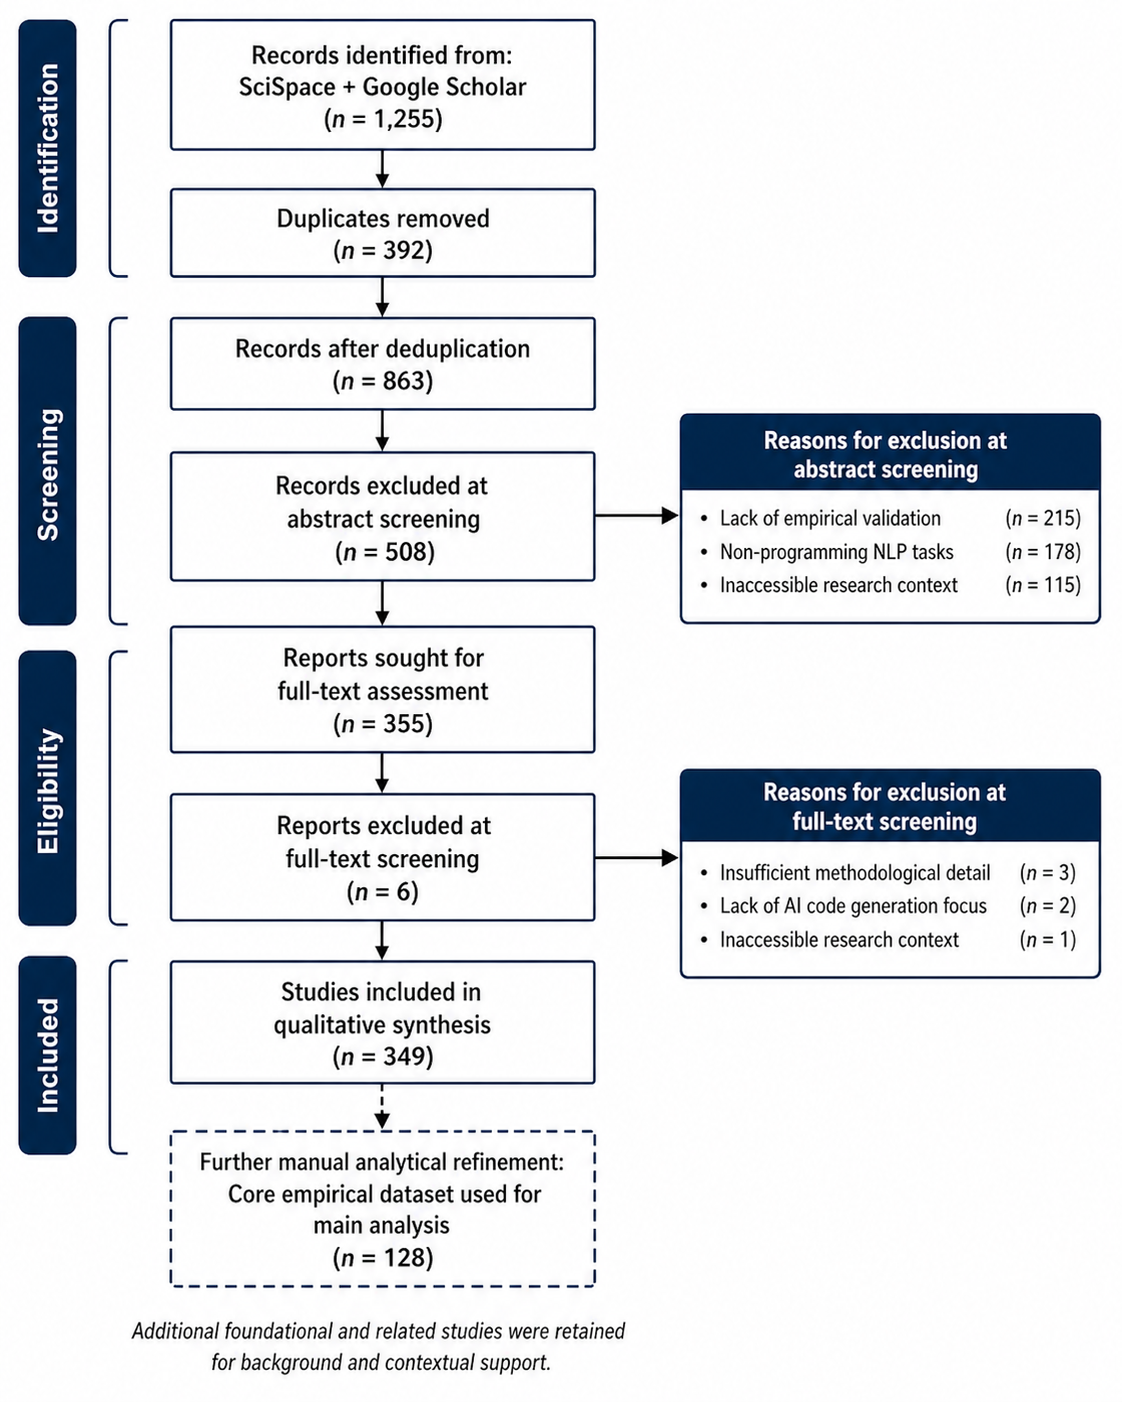
\includegraphics[width=0.9\linewidth]{figures/prisma_diagram.png}
    \caption{PRISMA flow diagram of the study selection process}
    \label{fig:prisma}
\end{figure}

\begin{table}[h]
\centering
\caption{PRISMA Study Selection Summary}
\begin{tabular}{l c}
\hline
Stage & Number of Studies \\
\hline
Initial records identified & 863 \\
After screening & 349 \\
After eligibility & 324 \\
Final included studies & 128 \\
\hline
\end{tabular}
\end{table}

The reduction from 324 eligible studies to 128 included studies reflects a final validation stage focused on quality filtering, removal of redundant or overlapping versions, and exclusion of studies with insufficient empirical grounding. This step ensured that the final dataset consisted of methodologically robust and non-duplicated evidence suitable for synthesis.

\section{Results}

\subsection{Overview of the Selected Studies}

After a multi-stage screening and validation process, a total of 100 studies were included in the final synthesis, comprising 98 primary studies and 2 secondary studies used for contextual and methodological support. The temporal distribution of the studies shows a strong concentration in recent years, with the majority published between 2024 (approximately 45\%) and 2025 (approximately 42\%), reflecting the rapid evolution of AI-assisted programming tools.

Regarding publication sources, the dataset includes a balanced mix of arXiv preprints (49\%), ACM venues (29\%), IEEE venues (13\%), and other verified publishers (approximately 9\%). This distribution indicates that, while the field is highly active, it is still partially consolidating in top-tier archival venues. These observations are derived from the selected studies included in this review..

\subsection{Research Methodologies (RQ6)}

The most common research methodologies identified were controlled experiments (34\%), observational studies (26\%), and mixed-methods approaches (10\%). Case studies and surveys together account for approximately 7\% of the selected studies.

These results suggest that the field is increasingly grounded in empirical evaluation, with a strong emphasis on experimental validation, consistent with trends observed in empirical software engineering research.

\subsection{Tool Coverage and Ecosystem (RQ1, RQ4)}

The literature is dominated by a small set of widely adopted tools, particularly GitHub Copilot (44\%) and ChatGPT (32\%). However, the dataset also includes emerging tools such as Gemini (7\%), Claude and Claude Code (7\%), OpenAI Codex (7\%), Amazon CodeWhisperer (6\%), and Tabnine (6\%), as well as additional tools including Cursor, Codeium, and DeepSeek-Coder.

This distribution highlights a transition from single-tool evaluations toward a more diverse ecosystem of AI-assisted development tools, as also reflected in prior comparative evaluations of multiple AI-assisted coding tools \cite{yetistiren2023evaluation}.

\subsection{Evaluation Metrics (RQ3)}

The most frequently used evaluation metrics include code quality (50\%), developer productivity or time savings (38\%), security and vulnerability analysis (30\%), accuracy and pass rates (20\%), and usability or developer experience (14\%).

These findings, derived primarily from empirical studies and supported by broader literature reviews, indicate that research has moved beyond productivity-centric evaluation to include multidimensional code quality assessments, alongside emerging security and risk considerations \cite{yetistiren2023evaluation, pearce2022security}.

Recent work has also introduced specialized metrics for evaluating bias in generated code, such as the Code Bias Score (CBS) and its multi-run variants, which capture both the prevalence and consistency of biased behaviors across model executions \cite{huang2025bias}.

To provide a structured overview of how key claims in the literature are supported by empirical evidence, Table~\ref{tab:evidence} summarizes the relationship between major findings, the type of evidence used, and the studies that support them. This mapping highlights the extent to which different dimensions—such as productivity, code quality, security, and developer experience—are grounded in empirical research.

\begin{table*}[t]
\centering
\caption{Summary of Evidence Supporting Key Claims in AI-Assisted Programming Research}
\label{tab:evidence}
\footnotesize{\textit{Strength} refers to the level of empirical support provided by the cited studies.}
\renewcommand{\arraystretch}{1.2}
\begin{tabular}{p{4.8cm} p{4.5cm} p{3.5cm} p{2cm}}
\hline
\textbf{Claim} & \textbf{Type of Evidence} & \textbf{Supporting Studies} & \textbf{Strength} \\
\hline

AI-assisted tools improve developer productivity & Controlled experiment (causal) & Peng et al. & Strong \\

Productivity gains vary by developer characteristics & Experimental (heterogeneous effects) & Peng et al. & Strong \\

AI-generated code is often correct or partially correct & Empirical code evaluation & Nguyen \& Nadi & Strong \\

Effectiveness varies across languages and problems & Experimental evaluation & Nguyen \& Nadi & Strong \\

AI-generated code may contain security vulnerabilities & Security analysis & Pearce et al. & Strong \\

Security risks require human validation & Empirical + inference & Pearce et al. & Strong \\

Performance varies across AI tools & Comparative empirical studies & Yetiştiren et al.; Idrisov \& Schlippe & Strong \\

Code quality is inherently multidimensional & Empirical + conceptual & Yetiştiren et al. & Strong \\

Correctness is measured via unit tests (pass@k) & Foundational methodology & Chen et al. & Strong \\

Multiple sampling improves correctness outcomes & Experimental evaluation & Chen et al. & Strong \\

AI-generated code is often understandable but imperfect & Complexity analysis & Nguyen \& Nadi & Strong \\

Productivity gains are context-dependent & Cross-study synthesis & Peng et al.; Vaithilingam et al. & Strong \\

No consistent productivity improvement across all scenarios & Human-subject experiment & Vaithilingam et al. & Strong \\

Developers prefer AI tools despite limitations & User study & Vaithilingam et al. & Strong \\

AI-generated code can be difficult to understand and debug & UX empirical study & Vaithilingam et al. & Strong \\

Over-reliance on AI suggestions is a risk & Behavioral observation & Vaithilingam et al. & Strong \\

AI tools function as starting points rather than final solutions & UX + empirical evidence & Vaithilingam et al.; Nguyen \& Nadi & Strong \\

Research employs diverse evaluation metrics & SLR synthesis & This study; Yetiştiren et al. & Moderate \\

The field is increasingly empirical & SLR synthesis & This study & Moderate \\

The AI tool ecosystem is expanding & Descriptive synthesis & This study & Moderate \\

Relationship between productivity and quality remains unclear & Cross-study synthesis & Peng et al.; Nguyen \& Nadi; Vaithilingam et al. & Strong \\

AI struggles with complex programming tasks & Experimental + synthesis & Chen et al.; Nguyen \& Nadi; Idrisov \& Schlippe & Strong \\

Maintainability varies across tools & Empirical evaluation & Yetiştiren et al.; Idrisov \& Schlippe & Strong \\

Efficiency metrics are part of evaluation frameworks & Empirical evaluation & Idrisov \& Schlippe & Strong \\

\hline
\end{tabular}
\end{table*}

\subsection{Impact on Productivity (RQ1)}

A substantial portion of the literature reports significant productivity improvements, particularly in tasks such as code completion, boilerplate generation, documentation, unit test generation, debugging, and other repetitive activities.

Reported gains commonly range between 30\% and 50\% time reduction, although results vary depending on task complexity and developer expertise, although results vary depending on developer characteristics such as experience and workload \cite{peng2023productivity}.

However, not all empirical evidence consistently supports these improvements. Controlled user studies have found no statistically significant differences in task completion time when using AI-assisted tools, particularly when generated code requires substantial debugging and validation \cite{vaithilingam2022usability}. Similarly, controlled studies of natural language-to-code assistants integrated within development environments report no statistically significant improvements in task completion time or correctness, despite positive user perceptions of the tools \cite{xu2022nl2code}.

Recent randomized controlled trials conducted in real-world development settings provide strong evidence that AI assistance does not universally improve productivity. In particular, experienced developers working on real tasks in large open-source repositories were found to take approximately 19\% more time when using AI tools, despite expecting substantial speed improvements \cite{becker2025impact}.

\subsection{Reported Benefits (RQ4)}

Beyond productivity improvements, the literature reports several additional benefits associated with AI-assisted programming tools. These include enhanced support for repetitive tasks such as code completion and documentation, improved accessibility for novice developers, and assistance in learning new programming concepts. Empirical studies also report that developers perceive AI-assisted tools as helpful and enjoyable to use, even in cases where objective performance improvements are not observed \cite{xu2022nl2code}.

AI tools are also frequently used to accelerate prototyping and reduce cognitive effort in routine coding activities. Additionally, developers report that such tools can serve as effective starting points for problem-solving, helping to generate initial code structures that can later be refined.

These benefits highlight the broader role of AI-assisted tools as supportive instruments that augment developer capabilities beyond simple efficiency gains.

\subsection{Code Quality and Reliability (RQ2)}

Despite productivity gains, the literature consistently identifies mixed effects on code quality. Positive outcomes are typically observed for small and well-defined tasks, particularly in terms of syntactic correctness. However, challenges arise in complex logic, multi-file contexts, and long-term maintainability. Empirical user studies further indicate that difficulties in understanding and debugging AI-generated code can negatively affect task effectiveness, particularly when developers must modify or repair code they did not originally write \cite{vaithilingam2022usability}. Additionally, empirical evaluations of in-IDE code generation and retrieval systems indicate that program correctness does not significantly improve with the use of such tools, further highlighting limitations in current AI-assisted development approaches \cite{xu2022nl2code}.

These findings are consistent with prior evaluations showing variability in correctness and maintainability across AI-generated code \cite{yetistiren2023evaluation}.

\subsection{Risks and Limitations (RQ5)}

The most frequently reported risks include security vulnerabilities in generated code, hallucinated or incorrect logic, over-reliance by developers, reduced understanding of underlying code, and inconsistent performance across programming languages and domains. Security-related concerns have been clearly documented in prior empirical work on AI-generated code \cite{pearce2022security}. Recent empirical studies conducted in real-world development environments further confirm that AI-generated code frequently contains security vulnerabilities. Large-scale analyses of code snippets from GitHub projects report that approximately 25--30\% of AI-generated code exhibits security weaknesses across multiple CWE categories, including high-severity vulnerabilities \cite{fu2025security}. 

In addition to security risks, emerging research highlights the presence of bias in AI-generated code across sensitive attributes such as age, gender, and region, with some models exhibiting biased behavior in a substantial proportion of generated outputs \cite{huang2025bias}. These findings expand the scope of risks associated with AI-assisted programming to include ethical and fairness considerations.

Notably, RQ5 is the most represented research question (approximately 73\%), indicating strong concern in the research community regarding safe and responsible adoption.

\subsection{Research Gaps and Trends (RQ7)}

The analysis reveals several key gaps in the literature, including the lack of standardized evaluation frameworks, limited longitudinal studies, underrepresentation of emerging tools such as Claude and Gemini, insufficient research on team-level and organizational impact, and scarcity of studies on long-term maintainability.

Interestingly, both developers and domain experts consistently overestimate the productivity benefits of AI assistance, highlighting a significant gap between perceived and actual performance improvements \cite{becker2025impact}.

These gaps suggest important opportunities for future research in AI-assisted software development.

\section{Discussion}

\subsection{Productivity Gains Are Real but Context-Dependent}

The results indicate that AI-assisted coding tools provide measurable productivity improvements, particularly in repetitive and well-defined tasks such as code completion, documentation, and testing \cite{peng2023productivity}. However, these gains are not uniform across all development activities. The effectiveness of such tools decreases as task complexity increases, especially in scenarios involving large codebases, multi-file dependencies, or domain-specific logic. These findings suggest that conclusions drawn from controlled or synthetic benchmarks may not generalize to real-world development environments, where task complexity, contextual knowledge, and integration overhead play a critical role.

This suggests that AI tools should be conceptualized not as replacements for developers, but as productivity amplifiers whose impact depends heavily on task structure and context. In particular, empirical studies of in-IDE natural language programming assistants suggest that improvements in developer productivity are not consistently observed, even when users report positive experiences with such tools \cite{xu2022nl2code}. This reinforces the notion that perceived usefulness does not necessarily translate into measurable efficiency gains. Furthermore, some controlled user studies report that while AI-generated suggestions can accelerate code production, they may also introduce additional debugging overhead, resulting in no significant net gains in task completion time \cite{vaithilingam2022usability}.

\subsection{Beyond Productivity: A Multi-Dimensional Evaluation Landscape}

While early discourse around AI coding assistants emphasized speed and efficiency, the current body of literature reflects a broader evaluation perspective. Code quality, security, maintainability, and developer experience are now central dimensions of analysis \cite{yetistiren2023evaluation}. Recent human-centered studies highlight that developer experience plays a critical role in the effectiveness of AI-assisted tools. While developers often perceive such tools as helpful and prefer to use them, they may struggle to understand, trust, and validate the generated code, particularly in more complex tasks \cite{vaithilingam2022usability}. This distinction between subjective user satisfaction and objective performance outcomes is also evident in studies of natural language-to-code systems, where developers express positive perceptions of the tools despite the absence of measurable improvements in productivity or correctness \cite{xu2022nl2code}. The discrepancy between perceived usefulness and actual productivity outcomes further reinforces the importance of distinguishing between subjective user experience and objective performance metrics.

In addition to traditional dimensions such as productivity and code quality, recent research highlights fairness as a critical evaluation dimension in AI-assisted programming. Empirical evidence shows that generated code may embed social biases, raising ethical concerns about the deployment of such systems in real-world applications \cite{huang2025bias}. Furthermore, studies indicate that simple prompt engineering techniques are often insufficient to mitigate bias, while feedback-driven approaches can significantly reduce biased behaviors in generated code \cite{huang2025bias}.

This integrated perspective is further reinforced by the structured synthesis presented in Table~\ref{tab:evidence}, which demonstrates how different claims are supported by complementary forms of empirical evidence. The table also highlights areas of convergence and divergence across studies, particularly regarding productivity outcomes, where both positive and neutral effects are reported depending on context.

\subsection{Dominance of Leading Tools and Emergence of New Ecosystems}

The literature remains dominated by GitHub Copilot and ChatGPT, which together account for the majority of empirical studies. However, the inclusion of tools such as Claude, Gemini, OpenAI Codex, CodeWhisperer, and others indicates the emergence of a more diverse ecosystem.

Despite their lower representation, these emerging tools are critical for understanding the evolution of AI-assisted development. Their inclusion helps mitigate bias toward a small number of widely studied platforms and provides a more comprehensive view of the technological landscape.

\subsection{Maturity of the Research Field}

Although the number of studies has grown rapidly, the field remains in a relatively early stage of consolidation. The high proportion of preprints suggests that research dissemination is still driven by speed rather than archival rigor.

This does not invalidate the findings, but it does imply that conclusions should be interpreted with caution. More rigorous empirical studies in top-tier venues are emerging, but further validation is still needed across diverse contexts and tools.

\subsection{Methodological Concentration and Its Implications}

The predominance of controlled experiments and observational studies indicates a strong empirical orientation. However, the lack of standardized evaluation frameworks limits comparability across studies.

This fragmentation creates challenges for meta-analysis and synthesis, as different studies employ heterogeneous metrics, datasets, and evaluation protocols. Addressing this issue represents a key opportunity for advancing the field.

Furthermore, the diversity of evaluation metrics identified in this study, as discussed in the Results section, highlights the absence of standardized measurement frameworks. This lack of consistency limits comparability across studies and complicates efforts to synthesize findings quantitatively.

These observations are consistent with broader systematic analyses of the field, which highlight structural challenges such as the lack of standardized benchmarks and heterogeneous evaluation practices across studies.

\subsection{Implications for Practice}

From a practical perspective, organizations adopting AI-assisted coding tools should consider both the benefits and limitations identified in the literature. While these tools can significantly reduce development time, they also introduce risks related to code quality and security.

Therefore, best practices should include:
\begin{itemize}
    \item Mandatory code review for AI-generated outputs
    \item Integration of security analysis tools
    \item Training developers to critically evaluate AI suggestions
\end{itemize}

\subsection{Implications for Research}

The findings highlight several directions for future research. These include the development of standardized evaluation methodologies, increased focus on longitudinal and real-world studies, deeper exploration of team-level impacts, and expanded investigation of emerging tools.

Additionally, there is a need to better understand how AI-assisted development affects software maintainability and developer cognition over time.

\subsection{Threats to Validity}

This study is subject to several limitations. First, the dataset includes a significant proportion of preprints, which may not have undergone rigorous peer review. Second, the reliance on automated screening tools introduces potential biases in study selection and scoring. Third, the diversity of evaluation metrics across studies limits direct comparability.

Despite these limitations, the systematic filtering, validation, and balancing procedures applied in this study provide a robust foundation for synthesizing current evidence in AI-assisted software development.

\section{Conclusion}

This paper presented a systematic literature review of AI-assisted programming in software engineering, focusing on the capabilities of current tools, their impact on developer productivity, and their influence on code quality. By analysing studies published between 2020 and 2026, this work provides a consolidated view of a rapidly evolving research area.

The findings indicate that AI-assisted programming tools offer substantial benefits in terms of productivity, particularly in tasks that are repetitive or well-defined. However, their impact on code quality remains less consistent. While efficiency improvements are frequently reported, they are sometimes accompanied by issues related to correctness, maintainability, and security. These results highlight the importance of balancing productivity gains with careful validation of AI-generated outputs.

Beyond summarising existing evidence, this study contributes by organising the literature into a structured framework and identifying key trends, limitations, and research gaps. In particular, the analysis underscores the need for more rigorous empirical studies, especially in real-world industrial contexts, as well as the development of standardised evaluation metrics.

Looking forward, AI-assisted programming is likely to play an increasingly central role in software development. Understanding how to effectively integrate these tools into development workflows, while mitigating their limitations, remains an important challenge for both researchers and practitioners. Continued investigation in this area will be essential to fully realise the potential of AI in software engineering.

\bibliographystyle{IEEEtran}
\bibliography{references}

\end{document}
